%\clearpage
\chapter{Etat de l'art}
\label{sec:SOTA}

L'idée de restreindre la gestuelle d'une personne à la seule dynamique de son ossature n'est pas nouvelle.
Durant les années 70, les travaux en psychologie de Johansson  \cite{johansson1973visual,johansson1976spatio} ont permis de montrer qu'avec seulement des points lumineux, l'être humain interprétait facilement les stimulis qui lui étaient présentés comme ceux d'un être humain effectuant des actions: l'humain peut donc reconnaitre une action juste avec la pose et sans information annexe telle que l'environnement. 

De ce fait, nous avons souhaité voir s'il était possible de réaliser l'analogie entre les travaux réalisés sur le stimuli humain et la machine.

\begin{figure}[H]
    \centering
    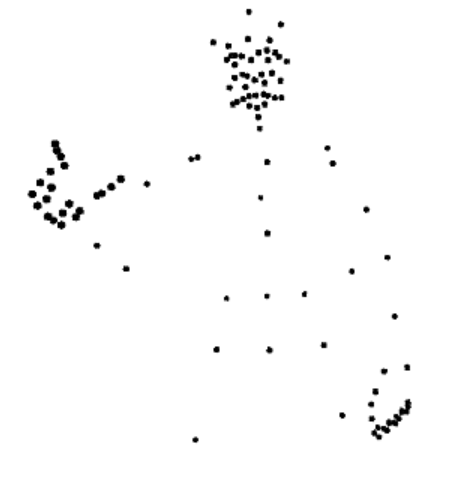
\includegraphics[width=0.34\linewidth]{Images/Johansson.png}
    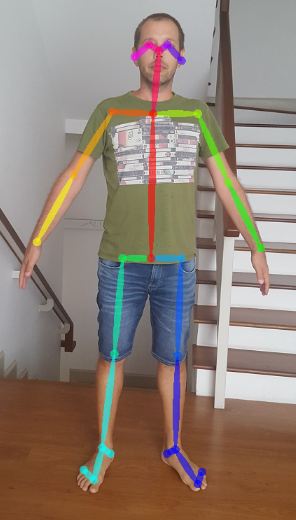
\includegraphics[width=0.2\linewidth]{Images/openpose2.png}
    \caption{A gauche: Un exemple de stimuli de l'experience de Johansson \cite{johansson1973visual,johansson1976spatio}.\\ A droite: la squelettisation obtenue après l'application d'Openpose \cite{cao2017realtime}}
    \label{fig:Johansson}
\end{figure}

Dans le cadre de cette thèse, nous cherchons dans un premier temps à lier la dynamique des articulations d'un piéton à une intention. Cette estimation de la dynamique des articulations sera ensuite combinée à la vision afin d’avoir une estimation plus robuste et absolue de l'intention du piéton en fonction de son environnement.\\





\section{Squelettisation de piétons}

Afin d’aboutir à cet objectif, la première étape essentielle est la détection et squelettisation des piétons. De nombreuses méthodes existent dans l’état de l’art, notamment par apprentissage profond où les récents résultats sont tout à fait prometteurs. La méthode finale ciblée concernant la prédiction des intentions raisonne sur la posture des piétons et nécessite donc d’être à même d’effectuer une extraction des articulations majeures des piétons en temps réel pour ensuite alimenter la phase de prédiction.


\begin{figure}[H]
    \centering
    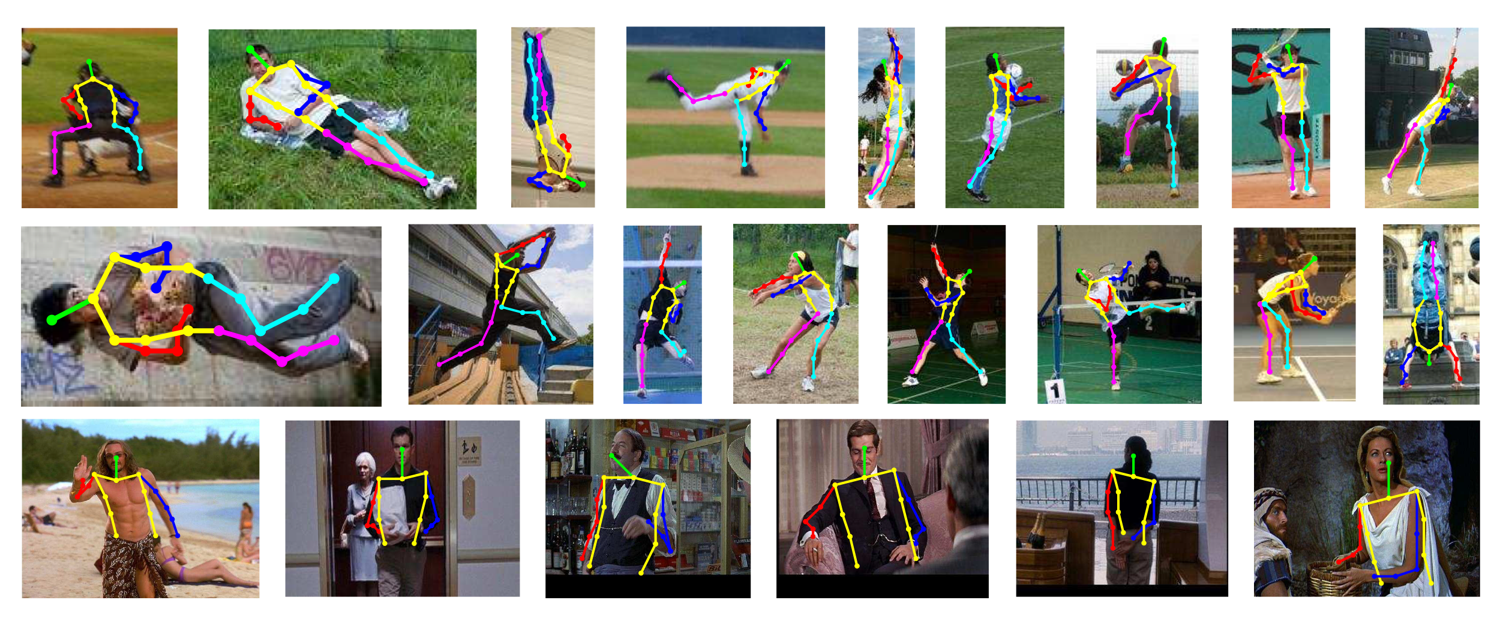
\includegraphics[width=0.9\linewidth]{Images/pose_estim_example.png}
    \caption{Exemples de squelettisations.}
    \label{fig:difficulte}
\end{figure}

L’objectif final étant orienté vers la prédiction des intentions, notre pipeline se basera sur des approches de l’état de l’art ayant démontré de bonnes performances et présentant des temps de calcul compatibles avec une utilisation temps réel.\\

La tâche de détection est compliquée de par la variabilité de l’apparence des personnes (vêtements, pose ...)
ainsi que par des phénomènes d’occlusions, dûs à la foule et au décor ou encore dûs à des problèmes d'echelle dans l'image.\\


\begin{figure}[H]
    \centering
    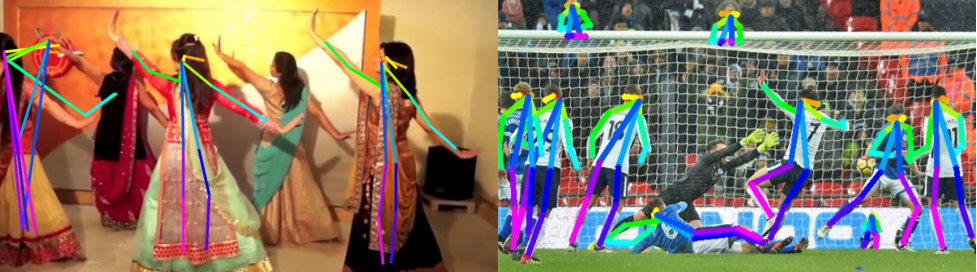
\includegraphics[width=0.85\linewidth]{Images/Difficulties.png}
    \caption{Exemple de cas difficiles pour des algorithmes de squelettisation: vêtements et luminosité à gauche, occlusion et échelle à droite.}
    \label{fig:difficulte}
\end{figure}
Ces difficultés sont l'une des causes de la recrudescence de l'intérêt des chercheurs pour traiter l'estimation de pose selon des approches d'apprentissage profond plutôt que par simple approche statistique comme cela était réalisé il y'a quelques années.\\

L'état actuel de la recherche dans ce domaine permet de discriminer les approches de squelettisation en deux types d'approches foncièrement différentes dans leur fonctionnement: ici définies comme les méthodes Top-Down et les méthodes Bottom-up.


\label{subsec:SQUEL}
\subsection{Approches Top Down}
\subsection{Approches Bottom Up}
\subsection{De la question de la dimension}

\section{Human Action Recognition}
\label{subsec:HAR}

La seconde étape de l'approche consistera en la classification des actions de la personne. La reconnaissance de l'action humaine dans une vidéo est un sujet de recherche difficile de par la grande variation et la complexité des données en entrée.

Les principales modalités utilisées pour la reconnaissance d'actions humaines comprennent les vidéos RGB dans leur intégralité \cite{donahue2015long,2014arXiv1412.0767T,varol2017long,Wu_2018_CVPR}, le flow optique \cite{simonyan2014two,zhang2016real,sevilla2018integration,DanutPOP} et la réprésentation sous forme de squelette \cite{vemulapalli2014human,du2015hierarchical,2016arXiv160707043L,2018arXiv180107455Y}.

Selon notre problématique: lier la dynamique de la pose à une classe, nous nous sommes majoritairement intéréssés à la dernière famille d'approches. La représentation sous forme de squelette qui semble être l'approche la plus robuste mais également la plus plausible pour une utilisation en temps réel:

\begin{itemize}
    \item En réduisant la taille des données d'entrée grâce à la structure de données associée aux squelettes, ce type d'approche est considéré comme bien plus rapide computationellement parlant que les modalitées listées précédement.
    \item Par ailleurs, celles-ci sont généralement bien plus robustes et capables de représenter les informations invarriantes d'une action puisque qu'aucun contexte de fond n'y est inclus.
\end{itemize}

La plupart des travaux existants dans la littérature se focalisent sur les approches basées sur la vidéo. Il existe à ce jour beaucoup moins de méthodes d'apprentissage traitant sur des données squelettiques comme entrée. Dans cette section, nous examinons une liste de ces approches basées sur l'apprentissage profond de reconnaissance d'actions sur des données squelettiques.

\subsection{Approches récurrentes}

Ces dernières années, les réseaux de neurones récurrents ont  été les approches de référence pour la modélisation de séquences en matière de reconnaissance vocale, de traitement numérique des signaux, de traitement vidéo et d'analyse des données textuelles. 


Analogiquement, la plupart des approches d'apprentissage profond pour la reconnaissance de gestes utilisent également des cellules récurrentes type LSTM \cite{hochreiter1997long} ou GRU \cite{2014arXiv1406.1078C}.

On représente le squelette sous forme d’une séquence et l'on y applique des réseaux de neurones à état, permettant de conserver l’information d’un instant de la séquence à un autre.

Ainsi, \cite{baccouche2011sequential} proposent une architecture combinant LSTM et RNN pour la reconnaissance d'actions.
 \cite{avola2018exploiting} exploitent les caractéristiques des angles de articulations apprises grâce à une architecture de type LSTM. 
\cite{zhang2017geometric} génèrent à partir des articulations, huit indicateurs géométriques et les évaluent avec un réseau LSTM à trois couches.
\cite{du2015hierarchical} divisent le squelette humain en cinq parties puis proposent une approche hierarchique séquentielle.
\cite{shukla2017recurrent} proposent une architecture récurente hierarchique sensiblement équivalente à \cite{du2015hierarchical} mais réduisent le nombre de articulations en entrée du modèle, certaines étant considérées comme superflues et ne portant que peu d'information. Conduisant à un ensemble réduit de paramètres et diminuant le temps d'inférence sans dégrader la qualité du classificateur.
\cite{shahroudy2016ntu} utilisent une approche LSTM se basant sur un apprentissage à long terme des cooccurrences d'articulations caractérisant intrinsèquement les actions humaines.
\cite{zhang2017view} proposent un réseau récurrent adaptatif avec une architecture LSTM, permettant au réseau de s'adapter aux points de vue d'observation les plus appropriés de bout en bout afin de gérer les grandes variations d'orientation dans les actions.

 

\subsection{Approches convolutives}
Les cellules récurrentes étant relativement lentes et difficiles à entrainer ainsi qu'à utiliser en temps réel comparé aux approches dites convolutives, celles-ci sont alors devenues une solution intéressante compte tenu de leurs avantages en matière de parallélisation, d'efficacité dans l'apprentissage des caractéristiques et de rapidité.


Les approches convolutives peuvent par exemple représenter le squelette sous la forme d'une pseudo-image pour appliquer des convolutions 2D, ou tout autre version spatio-temporelle des CNN comme les convolutions 3D. Les données squelettiques sont des éléments de faible dimension, il est donc envisageable d'organiser une séquence de caractéristiques du squelette de manière chronologique dans une image, qui conserve les informations originales de la dynamique du squelette.

\begin{figure}[H]
    \centering
    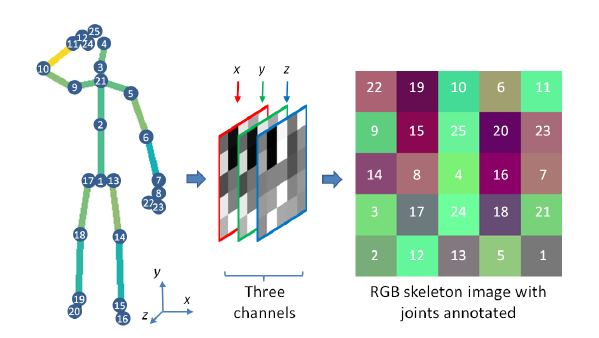
\includegraphics[width=0.7\linewidth]{Images/skeltoim.png}
    \caption{Organisation de la structure de données squelette en 3D en une image à trois channel (RGB)}
    \label{fig:skeltoim}
\end{figure}
L’idée générale étant de structurer les données pour leur donner la forme escomptée (une suite d’image) pour ensuite être classifiée en utilisant les méthodes standard de vision par ordinateur.\\


Ainsi, \cite{ke2017new} proposent de transformer une séquence squelette sous la forme de trois clips vidéos, les caractéristiques des CNN des trois clips sont alors fusionés en un unique vecteur de caractéristiques alors envoyé dans une softmax pour la classification.
\cite{pham2018learning} proposent d'utiliser un réseau résiduel \cite{he2016deep} avec pour entrée le squelette normalisé transformé dans l'espace RGB.
\cite{cao2018skeleton} proposent de classifier l'image obtenue grâce à des gated convolutions.
\cite{ludl2019simple} proposent une pipeline complète capable en temps réel de reconnaitre un humain dans une image, le squelettiser et déterminer l'action effectuée en utilisant le même format d'encodage sous forme d'image RGB.\\

En s'éloignant du domaine image mais en conservant la notion de convolution, d'autres approches à base de CNN les utilisent sous format 1D afin de modéliser des séquences:
\cite{bai2018empirical} montrent que les réseaux de convolutions peuvent égaler, voire surpasser les performances des réseaux récurrents pour des tâches typiques de modélisation séquentielle.\\

Par conséquent, \textit{ al.} \cite{devineau2018deep} proposent une architecture basée sur des convolutions parallèles capables de capturer des caractéristiques pour différentes résolutions temporelles.
\cite{2019arXiv190709658Y} proposent un modèle convolutif à trois branches prennant en entrée les positions des articulations du squelette à différentes vitesses et les distances par paires entre les articulations.
\cite{weng2018deformable} proposent un réseau de neurones déformable à convolution unidimensionnelle capable de découvrir les combinaisons d'articulations proteuses d'information et d'éviter les articulations dont la sémantique n'apporte que peu au modèle.



Les réseaux récurrents et les réseaux convolutifs peuvent également être fusionnés. L'approche consiste à extraire les informations spatiales avec des couches convolutives, puis de modéliser la dynamique temporelle par des couches récurrentes.

Ainsi, \cite{donahue2015long} proposent d'extraire les informations visuelles d'images provenant d'une vidéo grâce à un CNN 2D puis de les envoyer en entrée d'un LSTM.
\cite{li2017skeleton} proposent une approche où LSTM et CNN sont fusionnés "tardivement" (\textit{late fusion}). \cite{ullah2017action} proposent un approche bidirectionnelle où, les features obtenus par le CNN sont envoyés dans un LSTM bidirectionnel \cite{Schuster97bidirectionalrecurrent}, connectant deux couches cachées de directions opposées à la même sortie. La couche de sortie pouvant alors obtenir simultanément des informations sur les états passés et futurs.

\subsection{Attention}
La perception humaine se concentre sur les parties les plus pertinentes d'une image pour acquérir des informations permettant de comprendre la sémantique de celle-ci. Pour le machine learning, ce phénomène est artificiellement recréé  par le phénomène d'attention \cite{bahdanau2014neural,2017arXiv170603762V}: conceptuellement, l'attention peut être interprétée au sens large comme un vecteur de poids d'importance. 
Dans le cadre de la reconnaissance d'action, l'attention peut permettre de pondérer l'importance de certains instants de l'action pour la classifier ou encore pondérer l'importance de certaines articulations du squelette à l'instar d'autres articulations.
\cite{luong2015effective} distingue deux types d'attention: \textit{global attention} et \textit{local attention}:
 \begin{itemize}
     \item \textit{Local attention}: consiste en la suppression pure et simple de données lors de la selection des données d'entrée: les caractéristiques non pertinentes de l'environnement en dehors de la région considérée comme importante sont ignorées.
     \item \textit{Global attention}: consite en la prise en compte pondérée dynamiquement de l'ensemble des données de l'entrée.
 \end{itemize}
 
 %https://www.analyticsvidhya.com/blog/2019/11/comprehensive-guide-attention-mechanism-deep-learning/
 
 %https://lilianweng.github.io/lil-log/2018/06/24/attention-attention.html#a-family-of-attention-mechanisms

\cite{maghoumi2019deepgru} proposent d'empiler des GRU avec un mécanisme d'attention globale ainsi que deux couches entièrement connectées. \cite{song2017end} proposent un modèle à base de LSTM et de RNN et combinent attentions globales spatiale et temporelle. L'une capable de se focaliser sur les articulations discriminantes de chaque image et  l'autre pondérant les niveaux d'attention des résultats pour chaque instant afin de se focaliser sur les frames importantes. \cite{Fan2019AttentionBasedMR} utilisent les informations d'actions provenant de multiples points de vue afin d'améliorer les performances de reconnaissance et proposent un mécanisme d'attention pour la fusion multi-vues des squelettes envoyés à des LSTM. 

Il est également possible d'utiliser l'attention avec des convolutions.
Ainsi, \cite{hou2018spatial} proposent un réseau convolutif avec attention apprenant différents niveaux d'attention pour chaque caractéristique spatio-temporelle extraite par les filtres de convolution pour chacune des  frames de la séquence.

\subsection{Apprentissage géométrique profond}
L'évolution du squelette du corps humain au cours du temps peut être considérée sous la forme d'un graphe dynamique. Cependant, la recherche en apprentissage profond pour la reconnaissance d'actions sur des données squelettiques s'est jusqu'à présent principalement concentrée sur des données euclidiennes.
La nature non euclidienne de données sous format graphe rend l'utilisation d'opérations de base (comme la convolution) difficile à réaliser. 

Pour autant, l'utilisation de la structure de données format graphe pour un squelette lors de la classification d'actions humaines peut être intéréssante:

les convolutions ont par définition la capacité d'extraire des caractéristiques spatiales locales. Les structures de données type graphe sont adaptées puisqu'elles sont par définition, des structures connectées localement (l’ensemble des voisins d’un noeud). De cette manière, représenter le squelette sous la forme d'un graphe peut avoir l'avantage de ne pas exploiter des liens de voisinages entre joints inexistants mais de conserver une sémantique spatiale cohérente pour le squelette.

L'apprentissage géométrique profond (\textit{Geometric deep learning} voir par exemple \cite{gori2005new,scarselli2008graph,bronstein2017geometric}) désigne les techniques tentant de généraliser les réseaux de neurones profonds (structurés) à des domaines non euclidiens tels que les graphes. 

\cite{wu2019comprehensive} fournit un état de l'art sur l'apprentissage geométrique profond et propose une taxonomie pour différencier les reseaux géométriques en quatres catégories: récurrents, convolutionnels, auto-encodeurs et spatio-temporels.

Ainsi, \cite{2018arXiv180506184Z} proposent d'appliquer des convolutions sur les arêtes d'un graphe correspondant aux os du squelette afin de conserver la sémantique spatiale.
\cite{yan2018spatial} étendent les convolutions spatiales de graphe en convolutions spatio-temporelles. Ils proposent une approche spatio-temporelle convolutive incluant des articulations liées dans le temps dans le bloc convolutif en plus des articulations liées spatialement. \cite{2018arXiv180209834L} proposent de cumuler des convolutions spatio-temporelles avec un modèle ARMA (\textit{autoregressive moving average}). Finalement,  \cite{Si_2019_CVPR} proposent de cumuler l'attention à un réseau géométrique CNN-LSTM, capitalisant alors toutes les approches présentées précédement en un seul réseau.

\section{Prédiction d'intention}

\textbf{A ECRIRE}
\textit{La plupart des approches actuelles de la prédiction de l'action des piétons sont basées sur la trajectoire, ce qui signifie qu'elles s'appuient sur le mouvement passé observé des piétons et/ou la dynamique des véhicules pour prédire l'emplacement futur des piétons. Ces approches sont toutefois efficaces lorsque les piétons traversent déjà la rue ou sont sur le point de le faire: ces algorithmes réagissent à une action déjà en cours au lieu de l'anticiper.}


\textbf{Intéréssant}
\textit{In the literature various terms such as intention, actionand behavior are used to describe what the agent is doing or about to do in the scene. Here, we distinguish intention as the underlying state of mind which cannot be observed but can be inferred from the behavior. This is opposed toactions and, more generally, behaviors, i.e. observable ac-tions such as walking or crossing, for which there is groundtruth available.}




\subsection{Handcrafted}
\subsection{Apprentissage profond}


